\documentclass[journal,onecolumn]{IEEEtran}
\usepackage{booktabs,amsmath,graphicx,xcolor}
\newcommand{\rev}[1]{#1}
\begin{document}
\title{Supplementary Material for ``EASFL: Energy-Aware Federated Anomaly Detection in Wireless Sensor Networks With Mask-Aware Robust Aggregation''}
\author{Shiva~Kumar~V and~Choupiri~Shivakeshi}
\maketitle\renewcommand{\thetable}{S\arabic{table}}\renewcommand{\thefigure}{S\arabic{figure}}
All results are produced by the scripts in \texttt{simulator/} of https://github.com/vadlashiva/EASFL (branch \texttt{iotj-revision}); the file that produces each table is named in its caption.

\section*{S-A. Sensitivity, Unseen Fault Types, Detector Choice and Direction Test}

\begin{table}[h]\caption{Sensitivity of Lifetime and Energy to Network and Radio Parameters (Rounds; $E_{200}$ in J; Mean of 5 Seeds; \texttt{run\_sweeps.py}). --: Network Dead Before Round 200}\centering\small
\begin{tabular}{@{}llrrrr@{}}\toprule Setting & Scheme & FND & HND & LND & $E_{200}$\\\midrule
default & Centralized & 25 & 320 & 489 & 25.89\\
 & FedAvg-LEACH & 35 & 145 & 233 & 47.34\\
 & EASFL & 547 & 645 & 731 & 15.59\\
\midrule
$N=50$ & Centralized & 42 & 318 & 476 & 13.16\\
 & FedAvg-LEACH & 40 & 150 & 230 & 24.01\\
 & EASFL & 640 & 730 & 762 & 6.94\\
\midrule
$N=200$ & Centralized & 18 & 335 & 519 & 51.58\\
 & FedAvg-LEACH & 30 & 146 & 237 & 93.86\\
 & EASFL & 210 & 591 & 711 & 35.72\\
\midrule
field 200 m & Centralized & 4 & 121 & 292 & 43.22\\
 & FedAvg-LEACH & 20 & 73 & 159 & 49.63\\
 & EASFL & 488 & 560 & 604 & 17.49\\
\midrule
BS inside (50,50) & Centralized & 43 & 682 & 1178 & 13.08\\
 & FedAvg-LEACH & 34 & 189 & 300 & 42.10\\
 & EASFL & 561 & 761 & 823 & 13.51\\
\midrule
BS far (50,300) & Centralized & 1 & 33 & 71 & --\\
 & FedAvg-LEACH & 18 & 51 & 85 & --\\
 & EASFL & 191 & 221 & 294 & 45.58\\
\midrule
$p=0.05$ & Centralized & 34 & 318 & 478 & 27.81\\
 & FedAvg-LEACH & 46 & 159 & 251 & 46.30\\
 & EASFL & 629 & 777 & 792 & 13.14\\
\midrule
$p=0.2$ & Centralized & 26 & 323 & 485 & 26.11\\
 & FedAvg-LEACH & 29 & 128 & 218 & 48.25\\
 & EASFL & 142 & 563 & 713 & 19.63\\
\midrule
$E_{\mathrm{elec}}$ 25\,nJ/bit & Centralized & 28 & 408 & 599 & 20.99\\
 & FedAvg-LEACH & 47 & 206 & 351 & 40.06\\
 & EASFL & 903 & 992 & 1140 & 10.49\\
\midrule
$E_{\mathrm{elec}}$ 100\,nJ/bit & Centralized & 24 & 225 & 360 & 34.42\\
 & FedAvg-LEACH & 27 & 93 & 144 & --\\
 & EASFL & 281 & 395 & 444 & 25.84\\
\midrule
$e_s$ 0.5\,$\mu$J & Centralized & 25 & 320 & 489 & 25.89\\
 & FedAvg-LEACH & 35 & 157 & 253 & 46.10\\
 & EASFL & 561 & 752 & 906 & 13.24\\
\midrule
$e_s$ 8\,$\mu$J & Centralized & 25 & 320 & 489 & 25.89\\
 & FedAvg-LEACH & 33 & 116 & 178 & --\\
 & EASFL & 415 & 432 & 448 & 24.99\\

\bottomrule\end{tabular}\end{table}
Matched FedAvg (FedAvg with EASFL's compression, participation and CH policy) has the same lifetime as EASFL in every setting, because the aggregation rule has no radio cost.

\begin{table}[h]\caption{Recall per Fault Family When One Family Is Absent From the Training Windows (Synthetic, 5 Seeds; \texttt{run\_rev3.py e7}). Diagonal Entries Are the Held-Out Family}\centering\small
\begin{tabular}{@{}llccccc@{}}\toprule Scheme & Left out & Spike & Stuck-at & Drift & Burst & F1 (all)\\\midrule
Centralized & none & 0.56 & 1.00 & 0.88 & 0.68 & 0.812\\
 & Spike & \textbf{0.34} & 1.00 & 0.90 & 0.65 & 0.803\\
 & Stuck-at & 0.57 & \textbf{1.00} & 0.89 & 0.70 & 0.806\\
 & Drift & 0.56 & 1.00 & \textbf{0.51} & 0.69 & 0.752\\
 & Noise burst & 0.55 & 1.00 & 0.91 & \textbf{0.53} & 0.804\\
\midrule
EASFL-M, personalized & none & 0.58 & 1.00 & 0.89 & 0.72 & 0.830\\
 & Spike & \textbf{0.35} & 1.00 & 0.91 & 0.67 & 0.817\\
 & Stuck-at & 0.55 & \textbf{1.00} & 0.90 & 0.74 & 0.822\\
 & Drift & 0.60 & 1.00 & \textbf{0.51} & 0.73 & 0.771\\
 & Noise burst & 0.49 & 1.00 & 0.92 & \textbf{0.60} & 0.816\\

\bottomrule\end{tabular}\end{table}
\begin{table}[h]\caption{Detector Architectures, Centralized Training on Pooled Synthetic Windows (3 Seeds; \texttt{run\_detectors.py}), and Larger Federated Models (5 Seeds; \texttt{run\_rev3.py e12})}\centering\small
\begin{tabular}{@{}lrc@{}}\toprule Detector (input) & Parameters & Test F1\\\midrule
MLP 24-16-1 (features) & 417 & 0.782$\pm$0.013\\
Isolation forest (features) & -- & 0.656$\pm$0.024\\
1D-CNN autoencoder (raw) & 404 & 0.362$\pm$0.015\\
1D-CNN classifier (raw) & 1025 & 0.505$\pm$0.041\\
GRU classifier (raw) & 1025 & 0.629$\pm$0.029\\
\midrule Federated, 20\% sign flip & & Global F1 (clean / attack); alive at 200\\\midrule
MLP 24-80-1, EASFL-M & 2,081 & 0.694 / 0.475; 26 nodes, $E_{200}$=49.0\,J\\
MLP 24-80-1, Matched FedAvg & 2,081 & 0.652 / 0.177; 26 nodes, $E_{200}$=49.0\,J\\
MLP 24-400-1, EASFL-M & 10,401 & 0.560 / 0.134; 0 nodes, $E_{200}$=49.8\,J\\
MLP 24-400-1, Matched FedAvg & 10,401 & 0.588 / 0.182; 0 nodes, $E_{200}$=49.8\,J\\
\bottomrule\end{tabular}\end{table}
\begin{table}[h]\caption{Direction-Test Ablation Under Inner-Product Manipulation ($-0.5\Delta_i$) and Stealth Sign Flip ($-\Delta_i$) (Global F1, 10 Seeds; \texttt{run\_rev3.py e6})}\centering\small
\begin{tabular}{@{}lcccc@{}}\toprule Rule & IPM 20\% & IPM 30\% & Stealth 20\% & Stealth 30\%\\\midrule
Matched trimmed mean & 0.649$\pm$0.061 & 0.570$\pm$0.115 & 0.642$\pm$0.056 & 0.506$\pm$0.149\\
EASFL-M without direction test & 0.675$\pm$0.065 & 0.586$\pm$0.117 & 0.656$\pm$0.057 & 0.498$\pm$0.139\\
EASFL-M & 0.673$\pm$0.050 & 0.590$\pm$0.126 & 0.665$\pm$0.050 & 0.489$\pm$0.136\\
\bottomrule\end{tabular}\end{table}
\clearpage
% generated by apply_revision.py (stage 7): material moved from the main text
\section*{S-B. Packet Loss, Workload Sensitivity and Sampling Rate}
\subsubsection*{Packet Loss}
With packet-loss probabilities from 0 to 0.3, EASFL's global F1 stays between 0.69 and 0.72 and its personalized F1 at 0.82, whereas FedAvg-LEACH's global F1 falls from 0.69 to 0.65 at 30\% loss. Because each round aggregates many small, independent uploads, isolated losses mainly reduce the effective participation rather than biasing the update.

\subsubsection*{Sensitivity to the Synthetic Workload}
To verify that the conclusions are not artefacts of the generator settings, we varied the Dirichlet concentration $\alpha\in\{0.1,\dots,10\}$, the fault magnitude ($0.5$--$1.5\times$) and the anomaly rate ($0.5$--$2\times$). Fig.~\ref{fig:sens} shows that personalized EASFL matches or exceeds the centralized model in every setting except the smallest faults ($0.5\times$, where all methods reach only F1 $\approx0.54$ because faults are within noise), and stays within 0.02 of personalized FedAvg-LEACH throughout. Energy and traffic do not depend on the data, so EASFL's lifetime advantage is unaffected by these settings.

\begin{figure}[h]
\centering
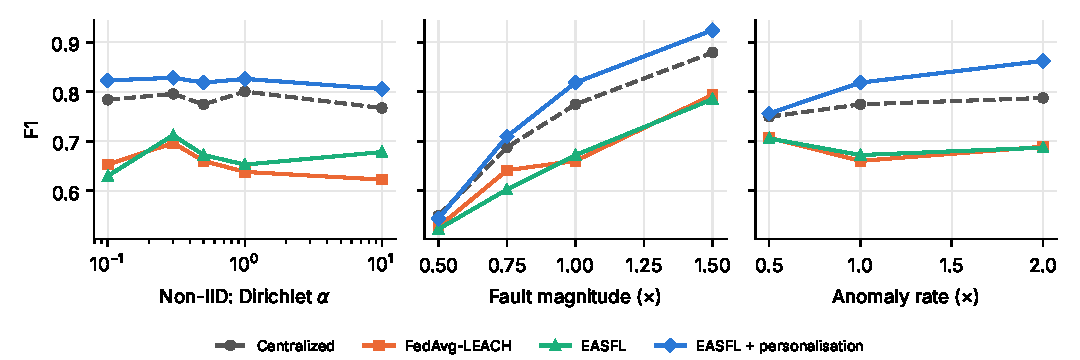
\includegraphics[width=\columnwidth]{figs/fig_sensitivity.pdf}
\caption{Sensitivity of F1 to the non-IID degree (Dirichlet $\alpha$), fault magnitude and anomaly rate (mean of 5 seeds).}
\label{fig:sens}
\end{figure}

\subsubsection*{When Is Centralized Collection Preferable?}
The energy of centralized collection grows with the raw sampling volume, whereas EASFL's communication does not. Varying the samples each node reports per round, centralized collection with LEACH achieves FND/HND of 81/1379 rounds at 10 samples, 45/589 at 30, 25/320 at 60 and 6/85 at 240. Hence, for very low reporting rates ($\le$10 samples per round) centralized collection outlives EASFL in HND, although its FND remains far shorter (81 vs.\ 547); above roughly 30 samples per round EASFL dominates on all lifetime metrics. The model size and the sampling rate together determine which design is preferable, and the cost model of Section~III of the main paper allows this crossover to be computed before deployment.


\section*{S-C. Energy Breakdown, CH-Policy Switching and Lifetime Detection}
\setcounter{table}{4}
\begin{table}[h]
\caption{\rev{Energy by Protocol Component Over 200 Rounds (J, Synthetic, Mean of 5 Seeds)}}\label{tab:s5}
\centering\scriptsize\setlength{\tabcolsep}{2.2pt}
\begin{tabular}{@{}lccccccc@{}}
\toprule
Scheme & Train & Uplink & CH rx & CH$\to$BS & Control & Broadcast & Total\\
\midrule
Centralized (raw) & -- & 5.49 & 3.23 & 17.32 & 0.93 & -- & 26.97\\
FedAvg-flat & 2.69 & 40.64 & -- & -- & -- & 6.08 & 49.41\\
FedAvg-LEACH & 4.37 & 14.09 & 9.20 & 9.75 & 0.81 & 9.86 & 48.06\\
EASFL-M & 3.15 & 0.43 & 0.43 & 2.51 & 2.19 & 6.87 & 15.59\\
\bottomrule
\end{tabular}
\end{table}
\begin{table}[h]
\caption{\rev{Effect of the CH Policy on Lifetime (Synthetic Network, 20 Seeds; Differences to Score-Based Selection, Paired)}}\label{tab:s6}
\centering\scriptsize\setlength{\tabcolsep}{3pt}
\begin{tabular}{@{}lcccc@{}}
\toprule
CH policy & FND & HND & LND & Node-rounds\\
\midrule
Score-based (EASFL) & 558 & 660 & 742 & 66{,}813\\
LEACH rotation & $-397$ & $+43$ & $+61$ & $-551$\\
Score + cooldown & $-227$ & $-34$ & $+33$ & $-4{,}094$\\
Switch at 10\% dead & 0 & $+5$ & $-6$ & $+98$\\
Switch at 50\% dead & 0 & 0 & $-4^{\ast}$ & $-36$\\
Switch at $\bar E<50\%$ & $-138$ & $+28$ & $-12^{\ast}$ & $+353$\\
Switch at $\bar E<25\%$ & $-19$ & $+18$ & $-13$ & $+674$\\
\bottomrule
\end{tabular}

\vspace{1mm}\parbox{\columnwidth}{\scriptsize All differences are significant at $p<0.05$ (Wilcoxon) except those marked $^\ast$. Node-rounds: sum over rounds of the number of alive nodes.}
\end{table}
\begin{table}[h]
\caption{\rev{Network-Level F1, Coverage and Cumulative Detection Over the Whole Lifetime With Learning Every Round (Synthetic, Mean of 5 Seeds)}}\label{tab:s7}
\centering\scriptsize\setlength{\tabcolsep}{1.5pt}
\begin{tabular}{@{}lccccc@{}}
\toprule
 & \multicolumn{4}{c}{Net F1 (coverage) at round} & Mean\\
Scheme & 200 & 400 & 600 & 800 & 1--1000\\
\midrule
Local only & 0.708 (1.00) & 0.685 (0.99) & 0.646 (0.95) & 0.547 (0.85) & 0.631\\
Centralized & 0.699 (0.75) & 0.380 (0.31) & 0 (0) & 0 (0) & 0.284\\
FedAvg-flat & 0.114 (0.08) & 0 (0) & 0 (0) & 0 (0) & 0.080\\
FedAvg-LEACH & 0.259 (0.23) & 0 (0) & 0 (0) & 0 (0) & 0.129\\
FedAvg, matched & 0.826 (1.00) & 0.831 (1.00) & 0.746 (0.82) & 0.027 (0.02) & 0.551\\
EASFL, dense & 0.821 (1.00) & 0.827 (1.00) & 0.666 (0.71) & 0.175 (0.10) & 0.567\\
\textbf{EASFL-M} & 0.827 (1.00) & 0.828 (1.00) & 0.741 (0.82) & 0.027 (0.02) & 0.551\\
\bottomrule
\end{tabular}
\end{table}
\section*{S-D. Detector Choice, Model Size and Thresholds}
\textit{Detector choice and model size.} On the pooled synthetic training data (centralized, 3 seeds; Supplementary Table~S3), the 417-parameter MLP on summary features (F1 0.78) outperforms an isolation forest on the same features (0.66), a GRU classifier with 1{,}025 parameters (0.63), a 1D-CNN classifier with 1{,}025 parameters (0.51) and a 1D-CNN autoencoder (0.36) on the raw 10-sample windows. Larger federated MLPs keep the robustness of EASFL-M (2{,}081 parameters: 0.48 against 0.18 for matched FedAvg under 20\% sign flip) but multiply radio energy: with 2{,}081 parameters only 26 of 100 nodes are alive at round 200, and with 10{,}401 none are. Model size, not only compression, must therefore be chosen against the energy budget.

\textit{Thresholds and personalization energy.} Choosing each node's threshold on a held-out 20\% validation split instead of its training windows lowers per-node F1 from 0.830 to 0.769, because fine-tuning and threshold selection then use fewer windows; the reported test F1 is computed on unseen test windows in both cases, so the training-window threshold does not inflate it. Personalization costs about 600 sample-passes (1.2\,mJ) per node once, 0.12\,J for the whole network, which is included in no table and is below 1\% of $E_{200}$.



\end{document}